\usecaseristoratore{Modifica ordinazione}
\label{usecase:Modifica ordinazione}

\begin{figure}[h]
	\centering
	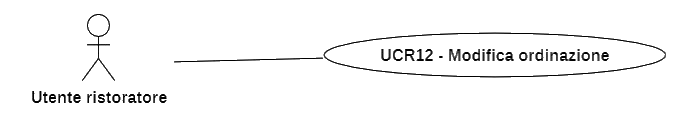
\includegraphics[width=0.9\textwidth]{./uml/UCR12.png} 
	\caption{Modifica ordinazione}
	\label{fig:UCR12}
  \end{figure}

\begin{itemize}

	\item \textbf{Descrizione:} Un Utente base ha un tempo limiato in cui può modificare il suo ordine, nel momento in cui lui voglia modificarlo ma ormai non sia più possibile, tale opzione di modifica è resa disponibile
	      attraverso la modifica dell'ordine da parte del ristoratore. L'utente può comunicare questa sua esigenza attraverso la \textit{chat} oppure di persona, e il ristoratore si prenderà cura di effettuare questa modifica.

	\item \textbf{Attore principale:} Utente ristoratore.

	\item \textbf{Precondizione:} L'Utente ristoratore sta visualizzando la lista delle ordinazioni di una prenotazione (vedi \autoref{usecase:Visualizzazione lista ordinazioni}).

	\item \textbf{Postcondizione:} L'Utente ristoratore modifica un ordinazione.

	\item \textbf{Scenario principale:}
	      \begin{enumerate}
		      \item L'Utente ristoratore viene a conoscenza della volontà
		            dell'Utente base di modificare il proprio ordine (vedi \textbf{Descrizione});
		      \item L'Utente ristoratore modifica l'ordine dell'Utente base:
		            \begin{itemize}
			            \item Modifica della quantità di una pietanza all'interno dell'ordine da modificare.
			            \item Rimozione di ingredienti di una pietanza all'interno dell'ordine da modificare.
			            \item Aggiunta di ingredienti di una pietanza all'interno dell'ordine da modificare.
		            \end{itemize}
		      \item Il Sistema notifica l'Utente base dell'avvenuta modifica al suo ordine (vedi \autoref{usecase:Visualizzazione notifica modifica ordinazione}).
	      \end{enumerate}

\end{itemize}
